\documentclass[a4paper,11pt]{article}
%% packages

\usepackage{blindtext} % needed for creating dummy text passages
%\usepackage{ngerman} % needed for German default language
\usepackage{amsmath} % needed for command eqref
\usepackage{amssymb} % needed for math fonts
\usepackage[colorlinks=true,breaklinks]{hyperref} % needed for creating hyperlinks in the document, the option colorlinks=true gets rid of the awful boxes, breaklinks breaks lonkg links (list of figures), and ngerman sets everything for german as default hyperlinks language
\usepackage[hyphenbreaks]{breakurl} % ben�tigt f�r das Brechen von URLs in Literaturreferenzen, hyphenbreaks auch bei links, die �ber eine Seite gehen (mit hyphenation).
\usepackage{xcolor}
\definecolor{c1}{rgb}{0,0,1} % blue
\definecolor{c2}{rgb}{0,0.3,0.9} % light blue
\definecolor{c3}{rgb}{0.3,0,0.9} % red blue
\hypersetup{
    linkcolor={c1}, % internal links
    citecolor={c2}, % citations
    urlcolor={c3} % external links/urls
}
%\usepackage{cite} % needed for cite
\usepackage[square,authoryear]{natbib} % needed for cite and abbrvnat bibliography style
\usepackage[nottoc]{tocbibind} % needed for displaying bibliography and other in the table of contents
\usepackage{graphicx} % needed for \includegraphics 
\usepackage{longtable} % needed for long tables over pages
\usepackage{bigstrut} % needed for the command \bigstrut
\usepackage{enumerate} % needed for some options in enumerate
\usepackage{todonotes} % needed for todos
\usepackage{makeidx} % needed for creating an index
\makeindex
%% page settings

\usepackage[top=2mm, bottom=15mm,left=5mm,right=5mm]{geometry} % needed for page border settings
\parindent=0cm % for space of first line of new text block
\sloppy % for writing with hyphenless justification (tries to)
\hyphenation{} % use hyphenation of tolerance parameters, http://www.jr-x.de/publikationen/latex/tipps/zeilenumbruch.html
\hyphenpenalty=10000
\exhyphenpenalty=10000
\usepackage{fancyhdr} % needed for head and foot options
%% my macros

%% Text fomats
\newcommand{\tbi}[1]{\textbf{\textit{#1}}}

%% Math fonts
\newcommand{\bbA}{\mathbb{A}}
\newcommand{\bbB}{\mathbb{B}}
\newcommand{\bbC}{\mathbb{C}}
\newcommand{\bbD}{\mathbb{D}}
\newcommand{\bbE}{\mathbb{E}}
\newcommand{\bbF}{\mathbb{F}}
\newcommand{\bbG}{\mathbb{G}}
\newcommand{\bbH}{\mathbb{H}}
\newcommand{\bbI}{\mathbb{I}}
\newcommand{\bbJ}{\mathbb{J}}
\newcommand{\bbK}{\mathbb{K}}
\newcommand{\bbL}{\mathbb{L}}
\newcommand{\bbM}{\mathbb{M}}
\newcommand{\bbN}{\mathbb{N}}
\newcommand{\bbO}{\mathbb{O}}
\newcommand{\bbP}{\mathbb{P}}
\newcommand{\bbQ}{\mathbb{Q}}
\newcommand{\bbR}{\mathbb{R}}
\newcommand{\bbS}{\mathbb{S}}
\newcommand{\bbT}{\mathbb{T}}
\newcommand{\bbU}{\mathbb{U}}
\newcommand{\bbV}{\mathbb{V}}
\newcommand{\bbW}{\mathbb{W}}
\newcommand{\bbX}{\mathbb{X}}
\newcommand{\bbY}{\mathbb{Y}}
\newcommand{\bbZ}{\mathbb{Z}}
\usepackage{url}
\usepackage{subfigure}
\usepackage{wrapfig}

\begin{document}
\begin{titlepage}
\center % Center everything on the page

%-------------------------------------------------------------------------------------
%	HEADING SECTIONS
%------------------------------------------------------------------------------------
\textbf{\large Department of Electronic and Telecommunication Engineering}\\[0.5cm]
\textbf{\Large University of Moratuwa, Sri Lanka}\\[1cm]
\textbf{\large EN2030 - Fundamentals of Computer Organization and Design}\\[2cm]

\includegraphics[width=0.3\textwidth]{uomlogo.png}\\[2cm]

	
%-------------------------------------------------------------------------------------
%	TITLE SECTION
%------------------------------------------------------------------------------------
\textbf{\Huge\underline {PROCESSOR DISSECTION}  }\\[2mm]
\textbf{\Huge\underline{REPORT}}\\[0.5cm]
\textbf{\Large Group 32}\\[5cm]


%----------------------------------------------------------------------------------------
%	MEMBERS SECTION
%----------------------------------------------------------------------------------------

\textbf{\large Submitted by}\\[0.5cm]
\begin{minipage}{0.32\textwidth}
	\begin{flushleft}
		{\large SIRITHUNGA M.R.A.	}\\[4mm]
		{\large SOMARATHNE P.M.P.H.	}\\[4mm]
		{\large THALAGALA B.P.		}\\[4mm]
	\end{flushleft}
\end{minipage}
\hspace{5mm}
\begin{minipage}{0.32\textwidth}
	\begin{flushright}
		{\large 180609B  }\\[4mm]
		{\large 180616T  }\\[4mm]
		{\large 180631J  }\\[4mm]
	\end{flushright}
\end{minipage}\\[2cm]


%----------------------------------------------------------------------------------------
%	DATE SECTION
%----------------------------------------------------------------------------------------
\textbf{\large Submitted on}\\[0.5cm]
\textbf{\large \today} % Date, change the \today to a set date if you want to be precise

%----------------------------------------------------------------------------------------

\vfill % Fill the rest of the page with whitespace

\end{titlepage}
\tableofcontents
\section*{\textbf{{Contribution from each member to the project}}}

\begin{table}[!h]
	\centering

		\begin{tabular}{|l|l|l|}
			\hline
			\textbf{Index}	&\textbf{Name} 	&\textbf{Contribution(Sections Covered)}\\ \hline
			&&\\
		180609B  	&SIRITHUNGA M.R.A. &* Micro-Architecture (Data Path and  Controller)\\
		&&* ALU functions\\ \hline&&\\

 		180616T  	&SOMARATHNE P.M.P.H. &* Instruction Set\\
 		&&*  Instruction classes and Instruction Format\\\hline&&\\

 		180631J		&THALAGALA B.P.&* Cache Memory and Memory Interfacing\\
 		&&*  Timing related to Memory\\\hline
		\end{tabular}

			\caption{Contribution from each member to the project}
\end{table}

\pagebreak

 \begin{figure}[!h]
	\centering
	\subfigure[Quad Core Core-i3 8300 Processor]
	{ 
\includegraphics[scale=0.15, angle= +90]{figures/soc}
			\label{intelsoc}
	}\hspace{1.5cm}
	\subfigure[A Single Core]
	{ 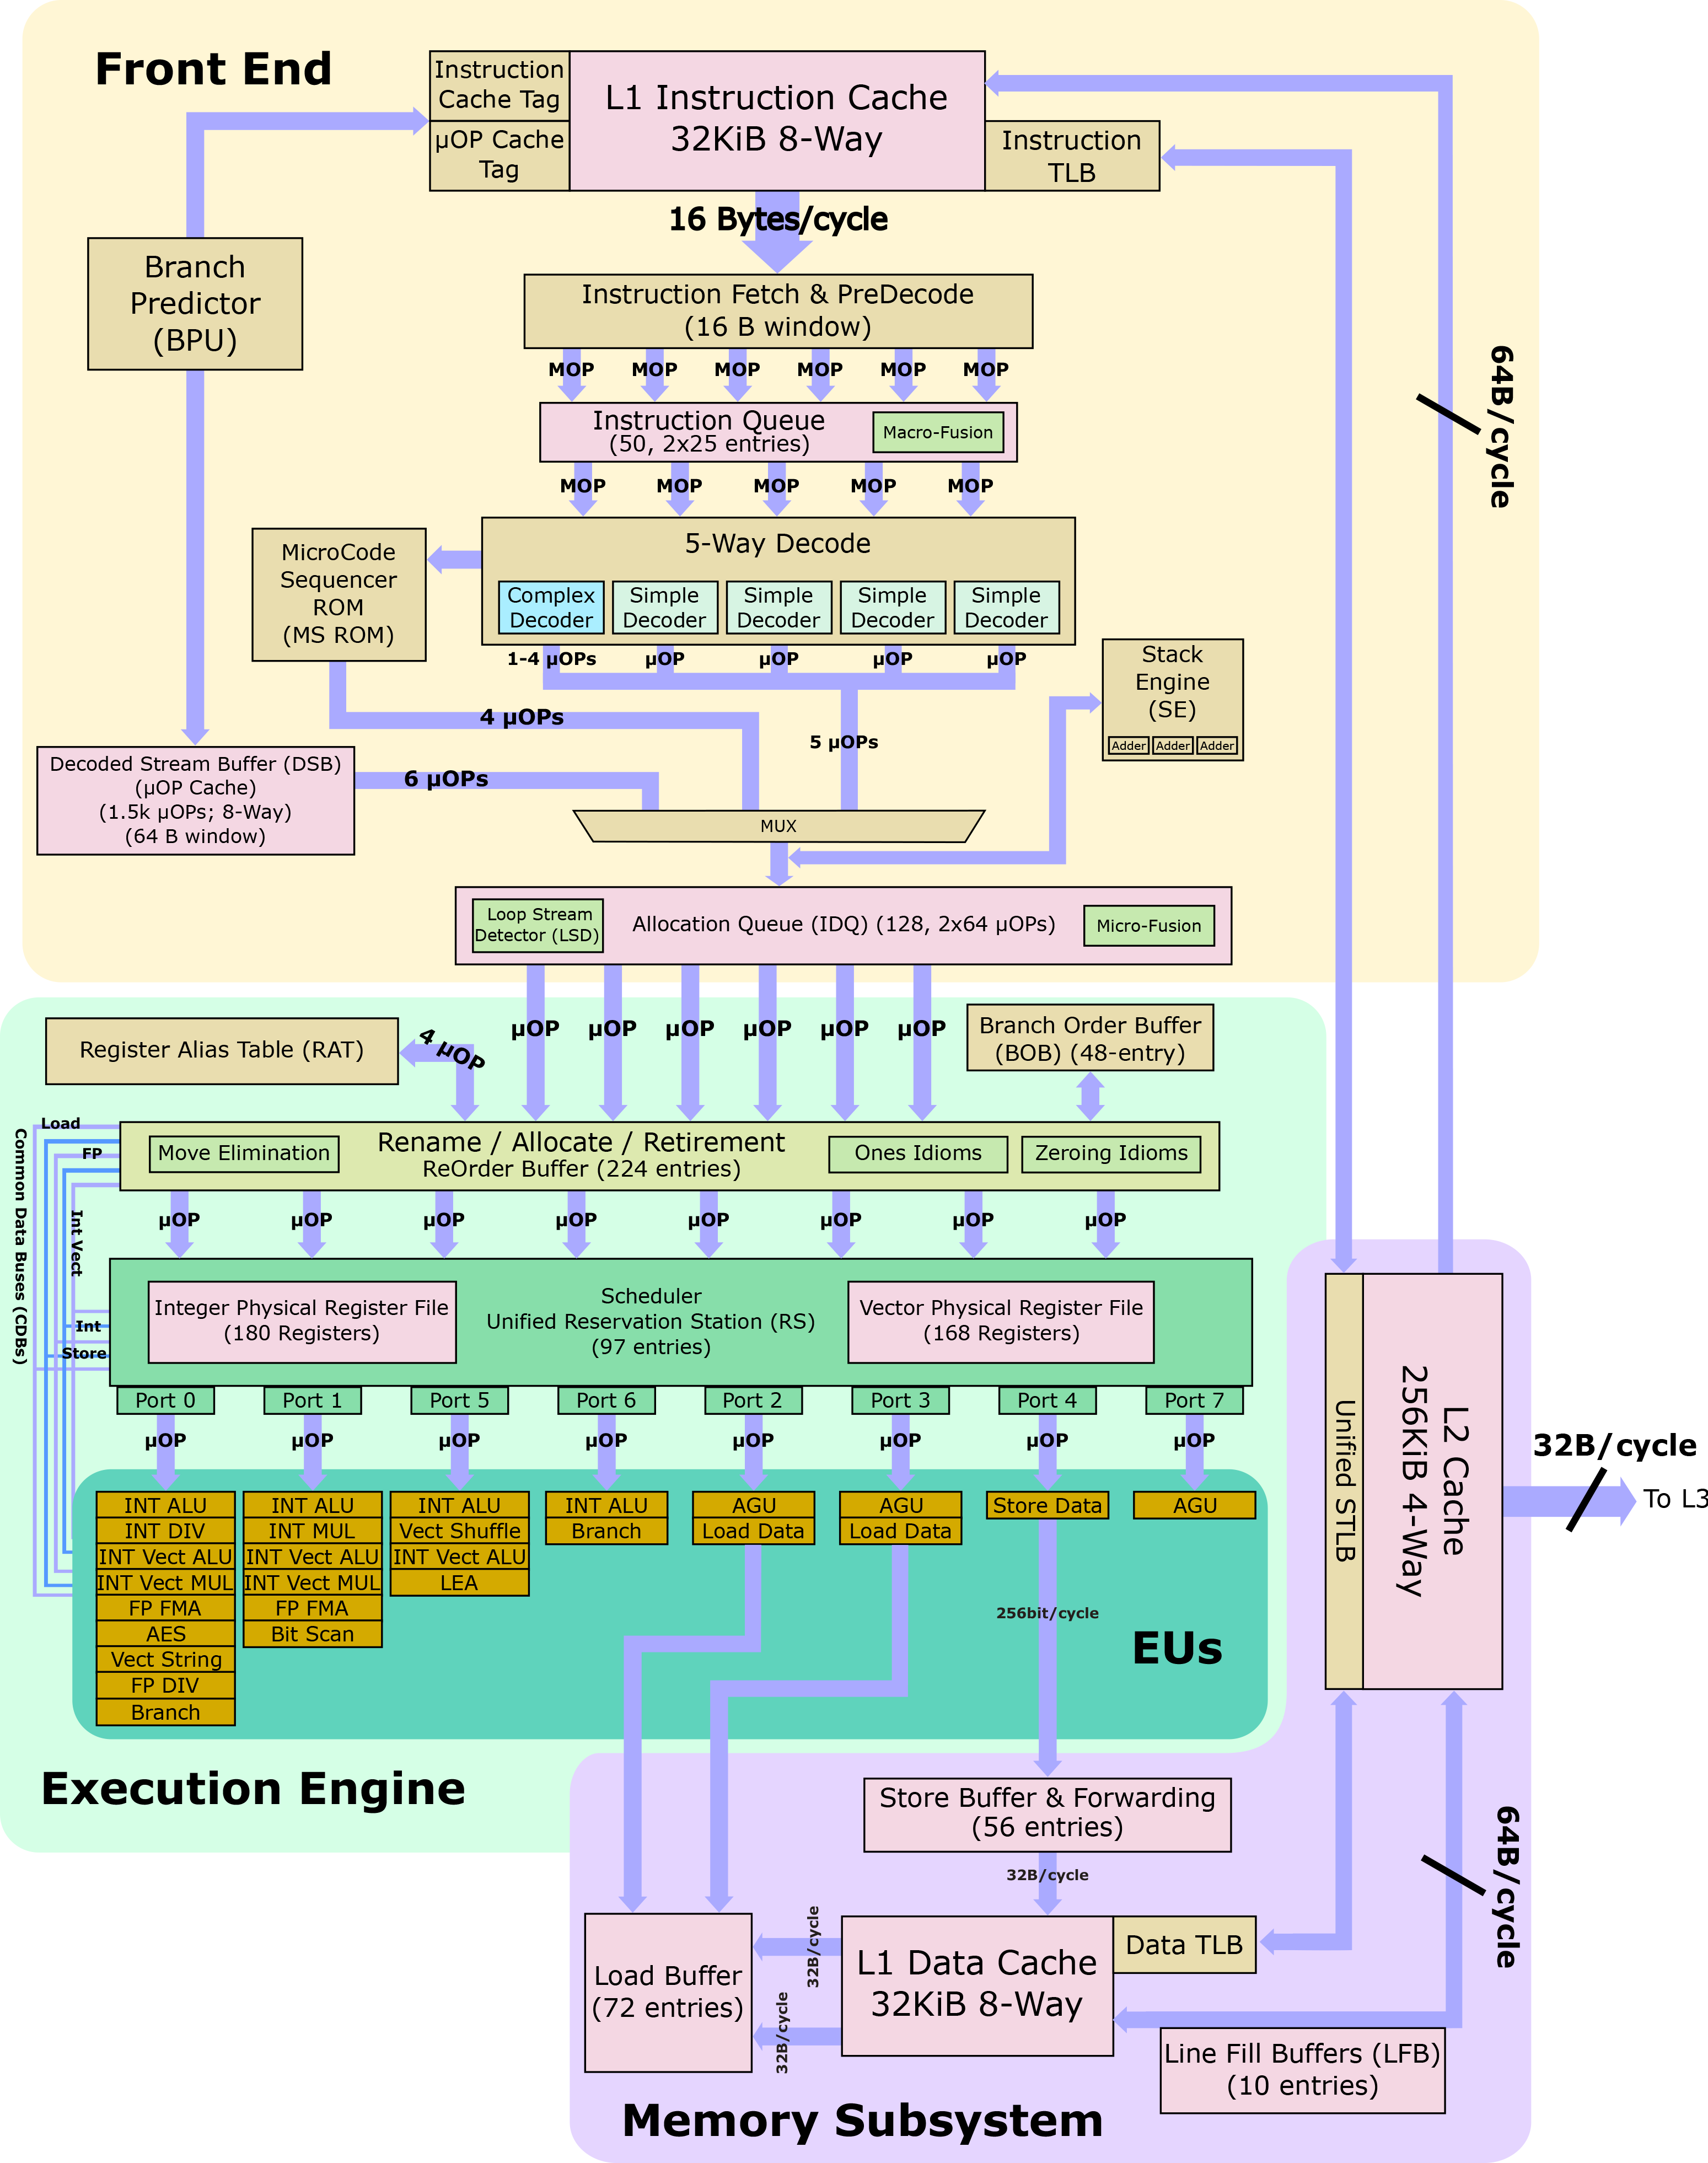
\includegraphics[scale=0.41]{figures/core}
			\label{intelcore}
	}
\caption{Intel core-i3 8300 Processor}
\end{figure}

 \begin{figure}[!h]
	\centering
	\subfigure[Dual Core - Cortex -R5 Processor]
	{ 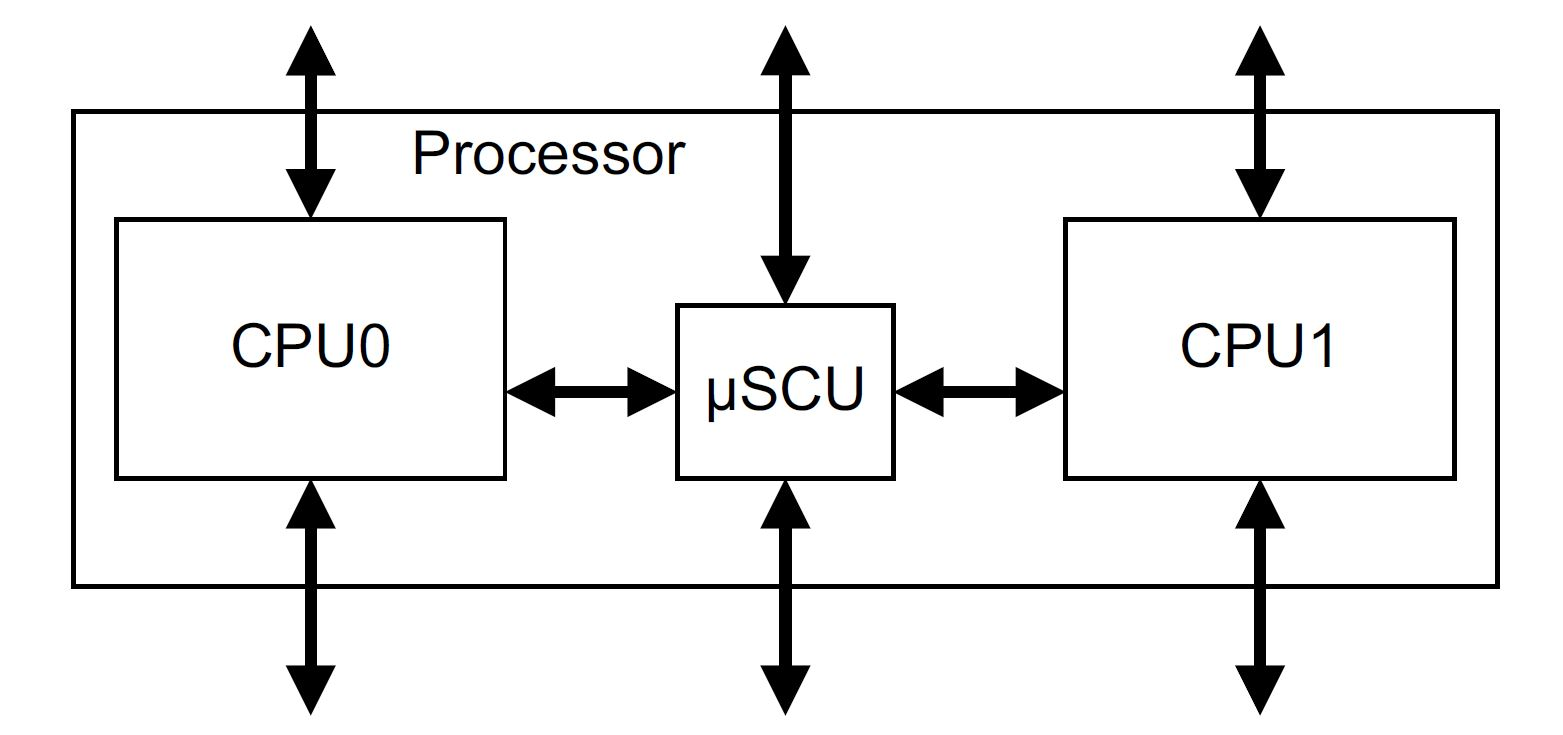
\includegraphics[scale=0.25, angle= +90]{figures/r5processor}
			\label{r5processor}
	}\hspace{1.5cm}
	\subfigure[A Single CPU]
	{ 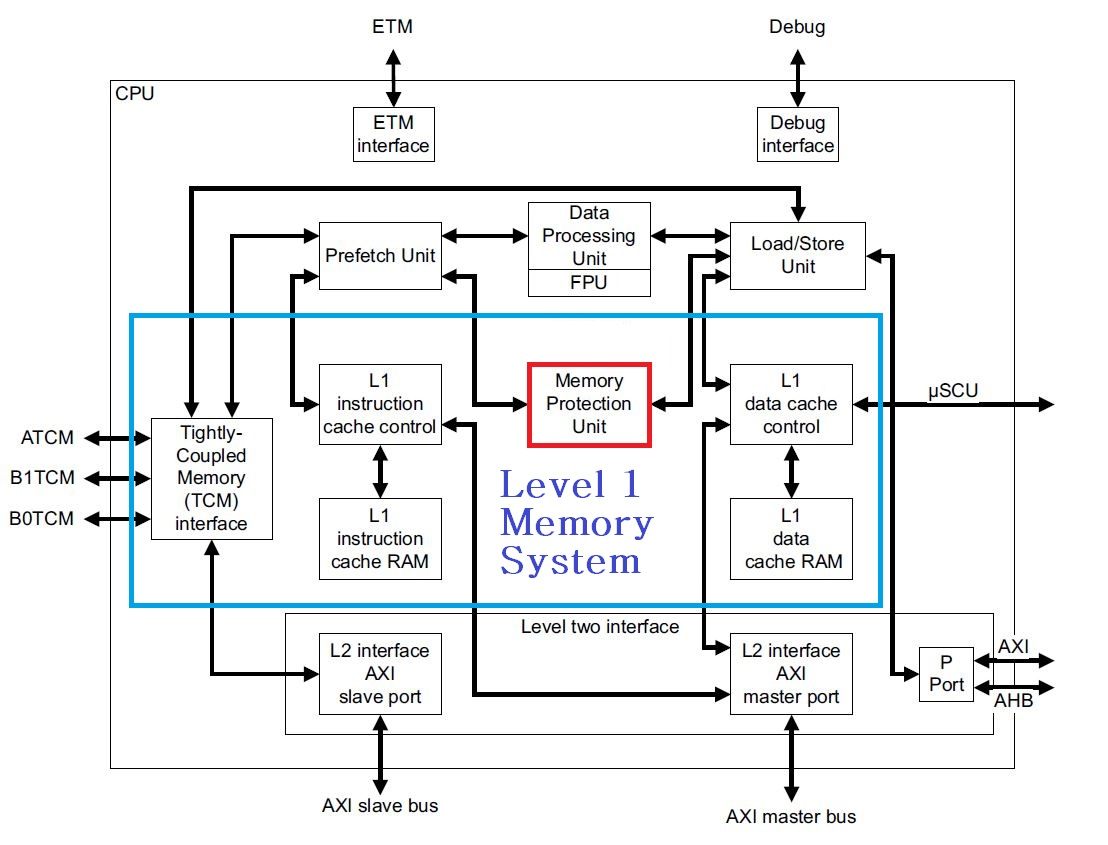
\includegraphics[scale=0.45]{figures/r5core}
	\label{r5core}
	}
\caption{ARM Cortex R5 Processor}
\end{figure}
\pagebreak

%============================================================
\section{Instruction Set Architecture of the Processor}

\subsection{Instruction Set}

\subsection{Instruction classes and Instruction Format}
glghuly

%=====================================================================
\vspace{1cm}\hrule

\section{Micro-Architecture (Data Path and the Controller)}
Computer architecture consists of two main branches called instruction set architecture (ISA) and microarchitecture ($\mu$arch). A given ISA can be implemented with different microarchitectures. So, microarchitecture depends on the ISA and the technologies used in implementations. The microarchitecture is the digital logic that defines the way of how the instructions should be executed. Here we have focused on the organization of the Data path and the controller of the internal processor design\cite{pcmag}.
\subsection{Arm Cortex-R5 Processor}
This is a mid-range CPU which is widely used in embedded, real-time systems. To that, ARMv7-R architecture is implemented in cortex-R5.ARM is a RISC architecture. Microcontroller Bus architecture has been embedded with it for better performance. When it comes to the internal design of the processor, the processor may have single or dual CPU configurations. However, the CPU data path is common at all 32bits data paths will be used\cite{TCLS}.(Refer figure \ref{r5core}) \\

The PreFetch Unit (PFU) fetches memory card instructions, predicts branches, and forwards the Data Processing Unit (DPU) instructions. Both directions are executed, and data memory is passed using the Load / Store Unit (LSU). The PFU and LSU interfaces support the L1 interface, which contains L1 instructions and caches, and TCM interfaces. In exchange, the L1 caches are linked to the L2 memory system and the LSU connects to the L2 memory system through a more direct peripheral port. Data Store interfaces L1 to the $\mu$SCU\cite{developer} for cache management to be compatible with ACP transactions.\\

\begin{figure}[!h]
	\centering
	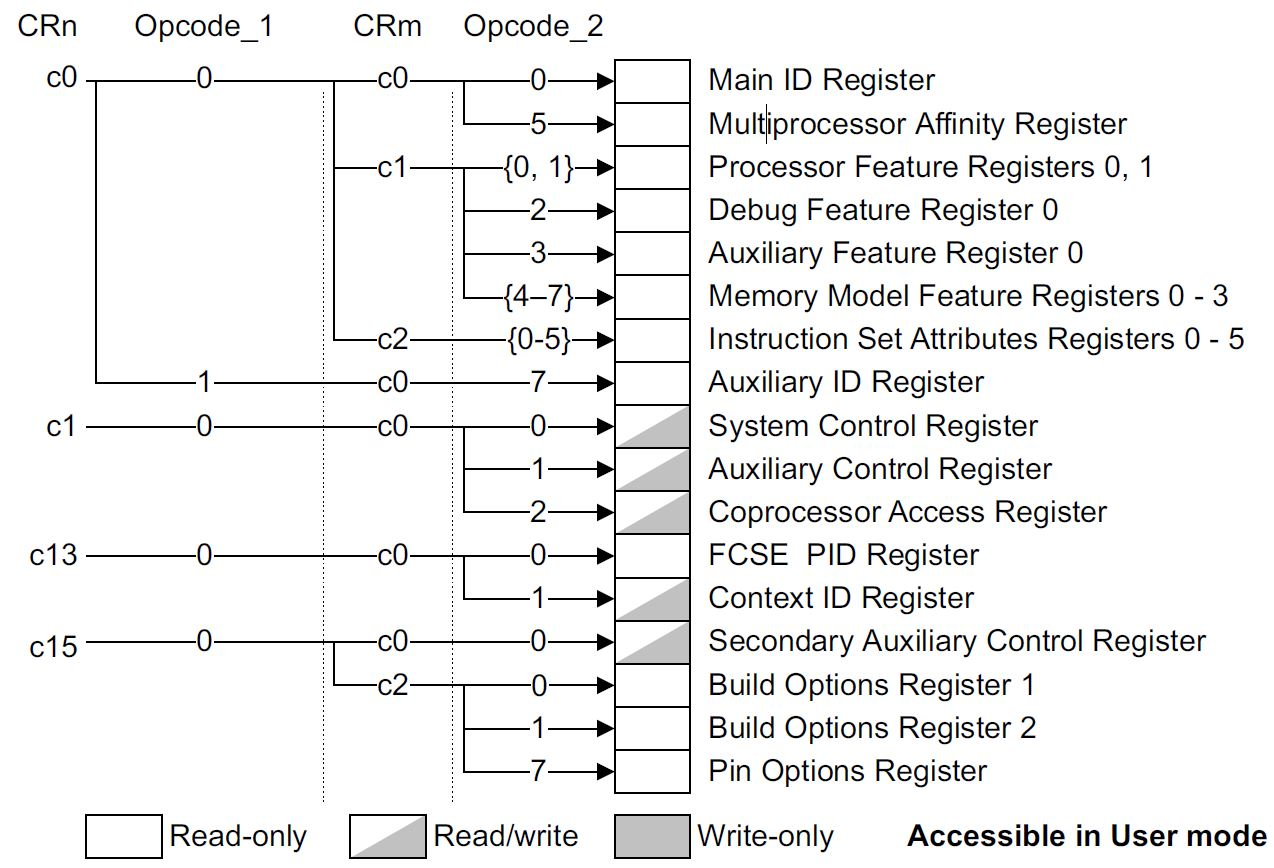
\includegraphics[scale= 0.3]{figures/syscc}
	\caption{System control and configuration registers}
\end{figure}

There is a system control coprocessor as the controller in cortex-R5 implementation.The control signals manipulating registers, device operations management of cache and the functionality of the memory system are induced by this. There are 18 read-only registers and 7 read/write registers among them as shown here.


\subsection{Intel Core i3-8300 Processor}
The internal design of an intel core i3 8300 is very advanced and complicated. It is CISC based microarchitecture called 'Coffee Lake'.  The actual size of a data path is 64 bits. Three levels of caches have been implemented inside it for better performance. Uni-processor configuration is used with four CPU cores and threads in the design. This is pipelined. The focus of the pipelining is to reduce power consumption and enhance overall performance. The coffee lake's pipeline is the same as intel's sky lake pipelining strategies. So, it is embedded in additional parallelism for achieving its performance. The pipeline can be split into three zones: the \textbf{\textit{front-end}}, \textit{\textbf{execution}}, and the \textbf{\textit{subsystem for memory}}. By encoding instructions, the front end is supposed to feed the back end with an appropriate stream of operations that it collects from memory. There are two major routes to the front-end: the micro-operations($\mu$OPs) cache route and the legacy path. The legacy path is the regular path by which x86 instructions of variable length are extracted, queued, and finally decoded into shorter fixed-length $\mu$OPs from the Level 1 instruction cache. The alternative and much more fitting solution is the cache route of $\mu$OPs in which a cache containing decoded $\mu$OPs receives a hit that explicitly passes the $\mu$OPs to the decode list.\\

\begin{wrapfigure}[15]{r}{3.7cm}
	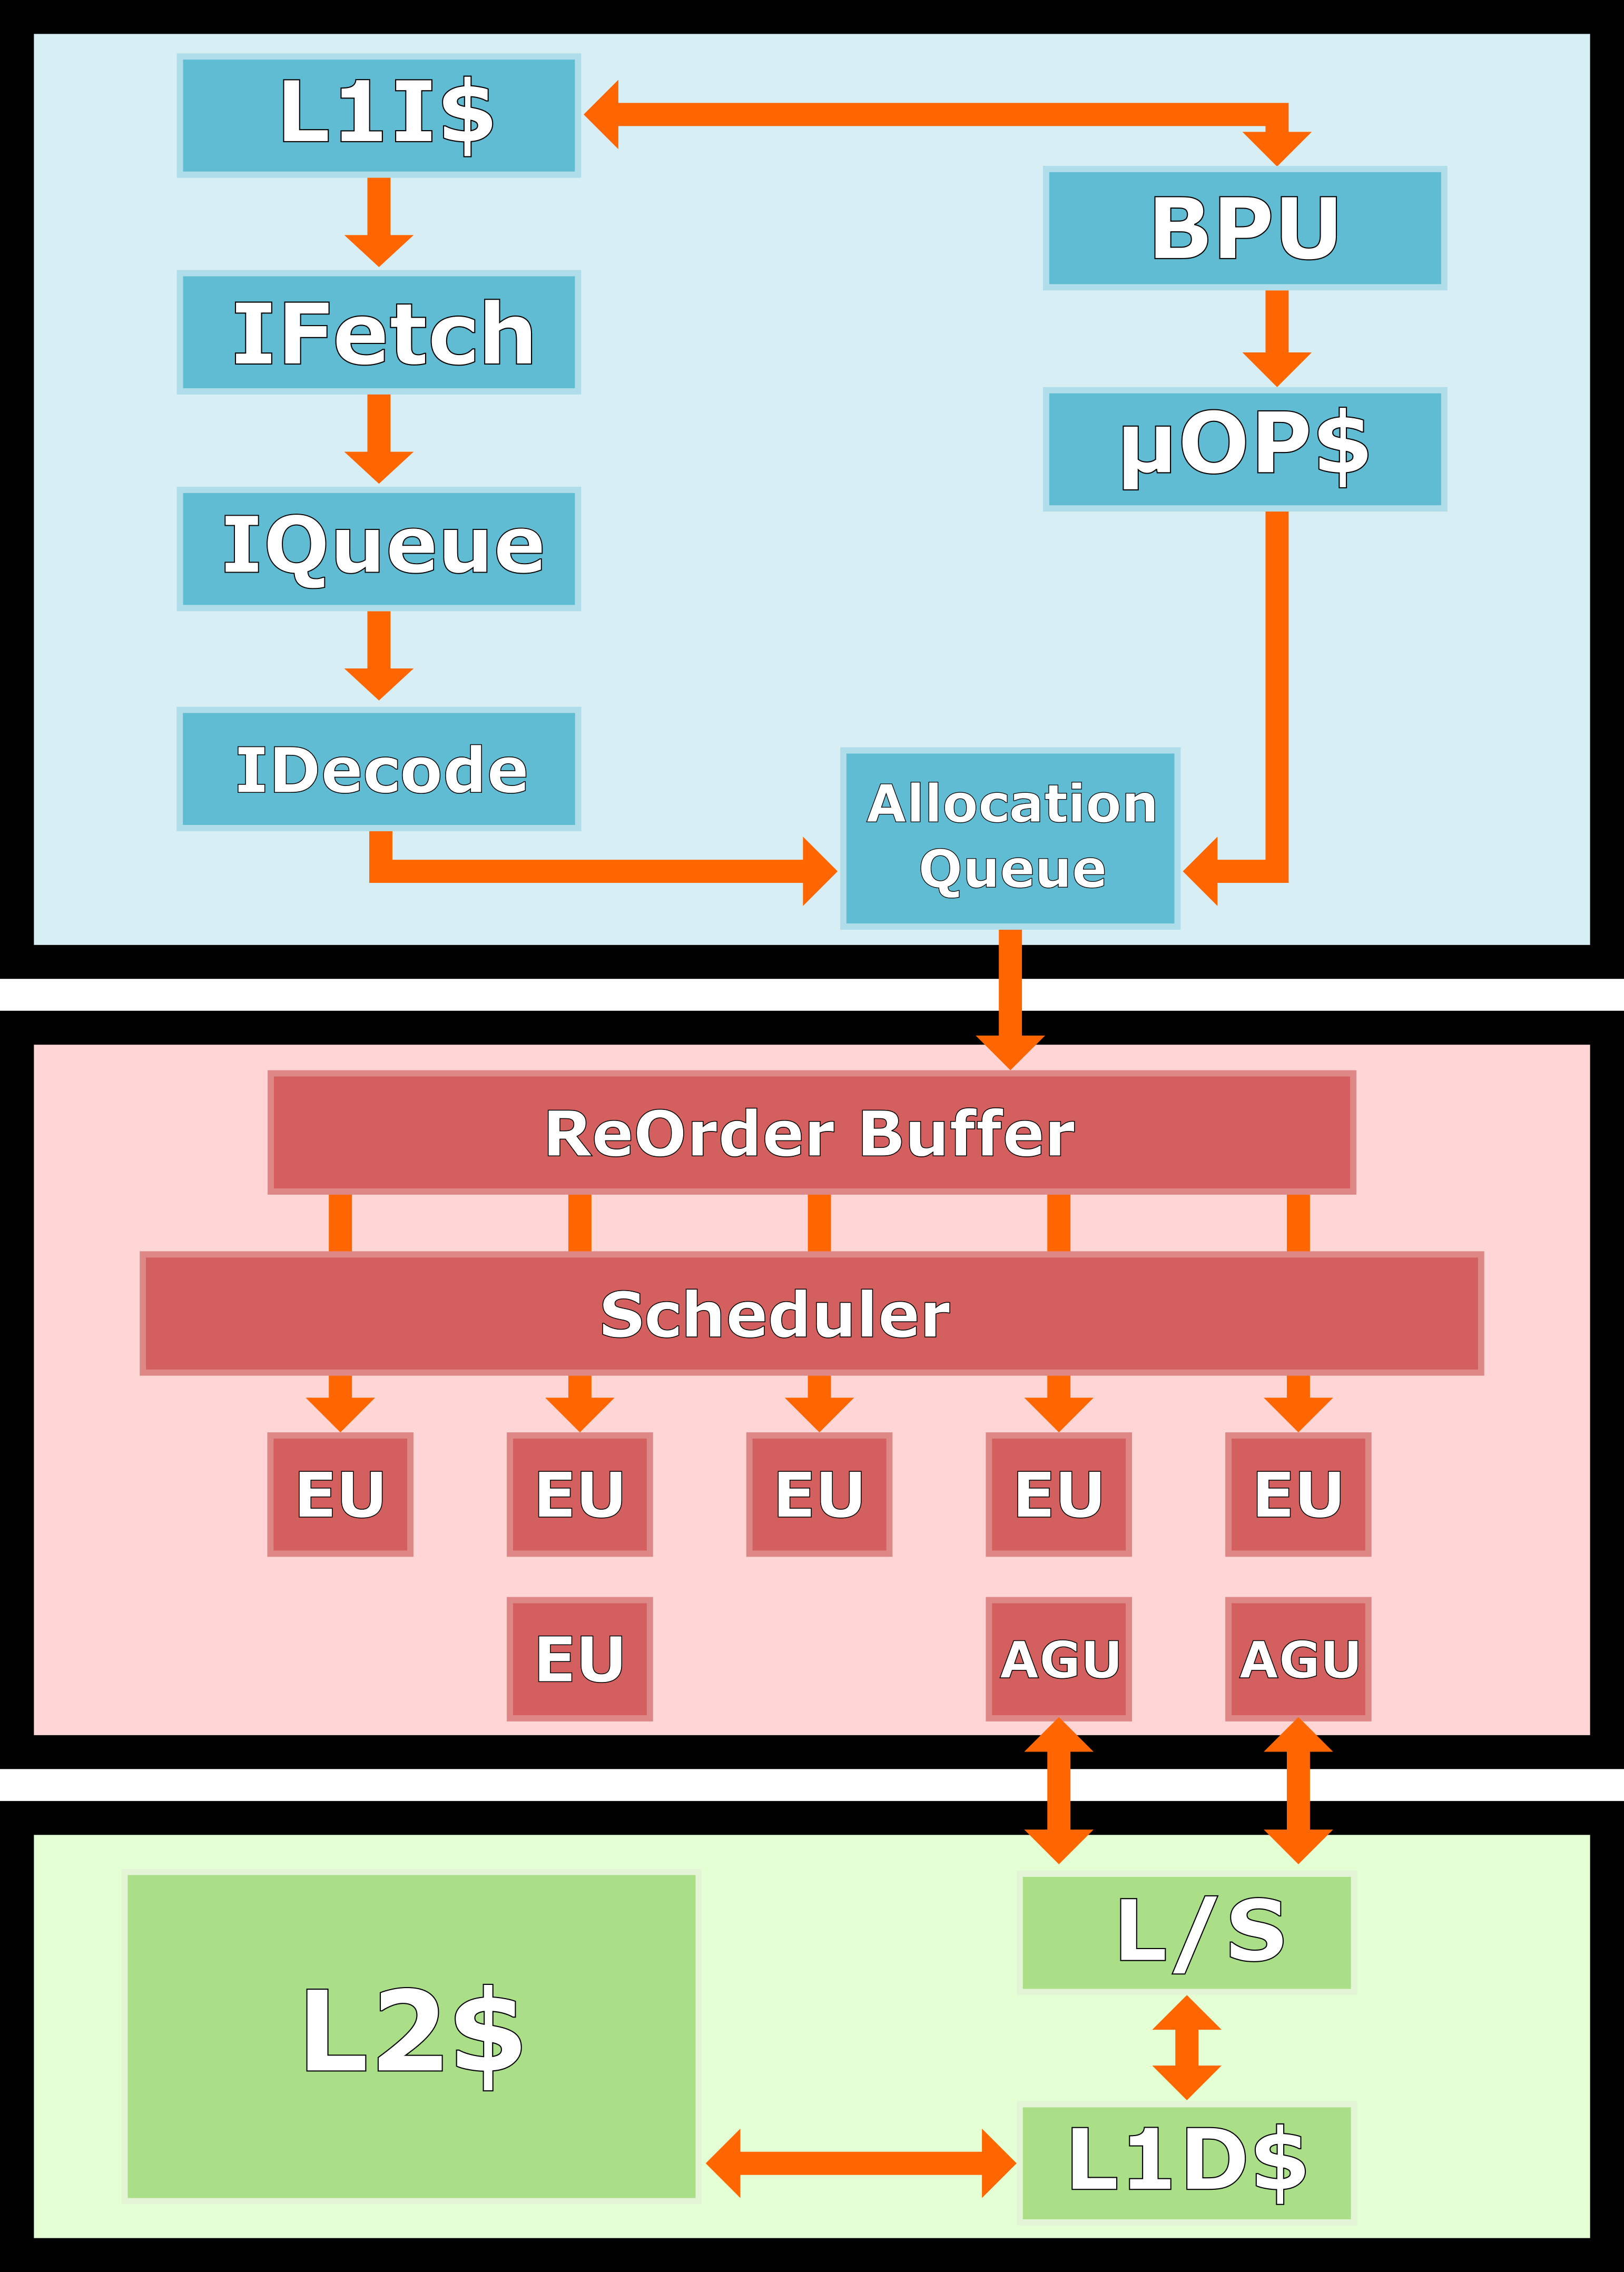
\includegraphics[scale= 0.05]{figures/intuarch}
	\caption{$\mu$arch: of Intel Core-i3 8300}
\end{wrapfigure}
The reorder buffer is visited at the back end by a micro-operation. This is where the register is reserved, renamed, and deleted. At this stage, several other optimizations are also carried out. The $\mu$OPs are forwarded to the unified scheduler from the reorder buffer. There are a few escape ports in the scheduler, each of which is connected to a set of distinct execution modules. Some units can perform basic ALU operations, others can multiply and divide, with some units, such as independent vector operations, capable of more complicated operations. The scheduler is responsible for the queuing of the $\mu$OPs to the relevant port so that the appropriate system will execute them.
Both $\mu$OPs deal with memory access, load \& store access. Those that can perform the memory operation would be sent to the dedicated scheduling ports. Store operations go to the buffer of the store, which is also able to forward if required. Mostly, load operations come from a load buffer.  According to that, the internal design consists of three major sub designs. These are focused on the following improvements,

 \begin{enumerate}[\hspace{1cm}1.]
 	\item \textbf{	Front end}
 	\begin{enumerate}[I.]
 		\item  	 Increase the delivery of the legacy pipeline to 5 micro operations.
 		\item Increase the spread of IDQ to 6 micro-operations.
 		\item Support for a 2.28x wider 64/thread allocation queue.
 		\item Improves the branch prediction unit's output.

 	\end{enumerate}

 	\item\textbf{	Execution engine}
 	\begin{enumerate}[I.]
 		\item  	 Increase the buffer for re-order to 224 entries.
 		\item Increase the scheduler to 97 entries and to 180 entries for the integer registry file.
 		\item Increase the buffer in the store to 56 entries.
 	\end{enumerate}

 	\item	\textbf{Memory subsystem}
 	\begin{enumerate}[I.]
 		\item Associative mapping, 8-way to 4-way set.
 	\end{enumerate}
 \end{enumerate}
The fetching and decoding of the instructions are happening separately. Fetched instructions are stored in a queue (FIFO). After decoding, these are executed in the execution engine.The control signals control each of these three subsystems. Generating control signals are done in a control store\cite{Coffee}.
\vspace{1cm}\hrule
\section{ALU functions}

The arithmetic and logic unit is abbreviated as ALU in the computer organization. ALU is responsible for all arithmetic and logical operations. It shall be carried out using the digital logic required for the respective set of operations.

 \begin{figure}[!h]
	\centering
	\subfigure[Core-i3 8300 Processor's ALU]
	{ 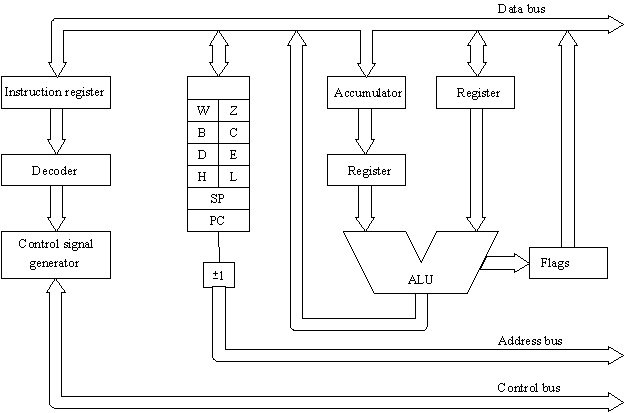
\includegraphics[scale=0.5]{figures/i3alu}
		\label{i3alu}
	}\hspace{1.5cm}
	\subfigure[Cortex-R5 processors's ALU]
	{ 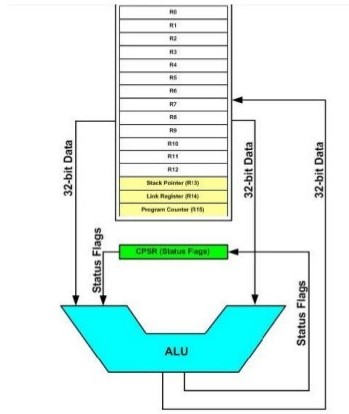
\includegraphics[scale=0.5]{figures/r5alu}
		\label{r5alu}
	}
	\caption{ALUs of the two processors}
\end{figure}

\subsection{Arm Cortex-R5 Processor}
In the eight-stage pipeline, an ALU performs its task. It two data paths that are directly connected with 32 bits registers. Cortex-R5 is well designed for digital signal processing and efficiently performed floating-point number calculations.(figure \ref{r5alu}) Four flags stand for,

\begin{itemize}
	\item 	N - Negative
\item	Z - Zero the ALU output subjected to NOR operation
\item 	C - Carry the Count bit
\item	V - Overflow V bit output
\end{itemize}

\subsection{Intel Core i3-8300 Processor}

Intel's Coffee Lake architecture is used 32bits registers. So, for that ALU should be capable of manipulating these numbers in it. This is achieved with digital logic. (figure \ref{i3alu}) Two of them are embedded in a processor for,
\begin{itemize}
	\item 	Physical address calculations
	\item	Mathematical operations

\end{itemize}

Core i3 processors are widely used in desktop and laptop general-purpose computers. The frequency of the clock is about 3.7 GHz, so the ALU operates at a higher speed than its clock time.\cite{howstuffworks}.


\vspace{1cm}\hrule
\section{Cache Memory and Memory Interfacing}

\subsection{Intel Core i3-8300 Processor}

\subsubsection{Memory Hierarchy}

\paragraph{Cache Memory}
Intel core i3-8300 processor's cache memory is organized using \textbf{\textit{Intel's Smart Cache}} technology. That is the Last Level Cache(LLC) is shared across all cores while lower level caches are separately allocated for each core such that those are used by the respective cores privately. The shared cache allows any of the four cores to access the entire storage area of the shared cache(\textit{in this case 8MiB LLC}) and therefore not limited to a dedicated portion of it. This leads to a number of benefits such as, increased resource utilization through providing all of the shared cache to the active cores if the other cores are in the idle mood, reduced front-side bus traffic since shared data can be fetched directly from the LLC(\textit{if available}) into the cores  rather than going all the way to the primary memory\cite{smartcache}.\\

 The following table summarizes the properties of each cache. Refer the \textit{memory subsystem} of the figure \ref{intelcore} to identify the organization of core-private caches while the shared cache(LLC/L3\$) is depicted inside the \textit{Ring} of the figure \ref{intelsoc}.\\

{\footnotesize \textit{Consider these abbreviations to refer tables},
D-\textit{Data}, I-\textit{Instruction}, WB-\textit{Write-back}, WT-\textit{Write-through} U-\textit{Unified}, S-\textit{Shared}, SA-\textit{Set Associative}}

 \begin{table}[!h]
	\centering
	\begin{tabular}{l| l |c |c |c|c}
		Cache  & Mapping Technology &Cache Size & No: of Sets&Cache line size& Writing Policy\\
		\hline
		L0 µOP Cache&8-way SA&1,536 µOPs&32&6-µOP&	N/A\\
		L1 I Cache &8-way SA&32 KiB&64&64 B&N/A\\
		L1 D Cache&8-way SA&32 KiB&64&64 B&WB\\
		L2 U cache&4-way SA&256 KiB&1024&64 B&WB\\
		L3 U, S Cache/LLC&Up to 16-way SA&8 MiB&8192&64 B&WB\\
		\hline\hline
	\end{tabular}
	\caption{Cache Memory Organization in Intel core i3-8300 Processors\cite{Coffee}}
\end{table}

\paragraph{Primary/Physical/Main Memory}
The next lower level memory after the L3 cache(LLC) is the System DRAM(Dynamic Random Access Memory) which is also known as the Primary/Main/Physical memory. Intel processors come in 4 different memory channel configurations as, \textit{Single channel, Dual channels, Triple channels and Flex mode}. Intel core i3-8300 Processor is a Dual channel and has the capability of reading from or writing to the primary memory in a maximum rate of  37.5GB/s. Moreover the processor supports up to 64GB of DDR4-2400 RAMs(the 4th generation of Double Data Rate(DDR) RAMs with 2400 Mbps data transfer rate) which is also an ECC(Error-Correcting Code) memory with the ability of detecting and correcting of common types of internal data corruptions.

\subsubsection{Translation-Lookaside Buffers(TLBs)}
In a \textit{\textbf{Virtual Memory System Architecture}}(VMSA)(the technique of using primary memory as a cache for the secondary memory) the processor generates \textit{virtual addresses} while the memory is accessed using the \textit{physical addresses}. The mechanism of translating a virtual address to a physical address is called \textbf{\textit{Address Translation/ Mapping}} and it consumes time. Because a single memory access in such a virtual system is actually a two physical memory accesses: first access to obtain the physical address corresponding to the virtual address from the \textit{page table}(part of the memory where physical addresses corresponding to virtual addresses are stored) and the second access to obtain the required data stored in that physical address.\\

To reduce this latency, an address-translation cache which is known as \textbf{\textit{Translation-Lookaside Buffer(TLB)}} where recent address translations are stored is used. In a single core of the Intel core i3-8300 Processor there are three TLBs and their properties are given in the following table while the physical placement is shown in the \textit{Memory Subsystem} and the upper part of the \textit{Front End} of the figure \ref{intelcore}.


\begin{table}[!h]
	\centering
	\begin{tabular}{l |l| c| c| c}
		TLB  & Mapping Technology & Page size & No: of Entries& Partitioning Method\\
		\hline
		I-TLB & 8-way SA & 4 KiB& 128 &Dynamic\\
		D-TLB &  4-way SA & 4 KiB &64 &Fixed\\
		STLB U & 12-way SA&  4 KiB + 2 MiB & 1536 & Fixed\\
		\hline\hline
	\end{tabular}
	\caption{TLBs Organization in Intel core i3-8300 Processors}
\end{table}


\subsubsection{Store Buffers}

Each core of an Intel Core-i3 processor consists of a Store Buffer, which is located between the \textit{Port 4}(dedicated port for storing data) of the scheduler and the \textit{L1-Data cache} as shown in the figure \ref{intelcore}. Every \textbf{\textit{memory write}} operation carried out by the processor is temporarily stored in this buffer before they are executed. So the processor does not have to wait until the operation is finished and it can carry out the rest of the instructions freely. This mechanism increases the processor's overall performance through \textit{\textbf{eliminating the unwanted idling}}.
%11.1 INTERNAL CACHES, TLBS, AND BUFFERS


%==================================================================================

\subsection{Arm Cortex-R5 Processor}

\subsubsection{Memory Hierarchy}

\paragraph{Cache Memory} Arm Cortex-R5 Processor's CPUs only have Level 1(L1) integrated cache controllers while ARM-L2 cache controllers can be connected outside of the processor instance according to the requirement, by the system designer. L1 caches are split as \textit{L1 Instruction cache} and \textit{L1 Data cach}e in order to increase the performance through increasing the bandwidth. Moreover, their sizes can be independently configured to be between 4KB and 64KB and each cache can be disabled independently. Data and Instructions are fetched in to the L1 caches via the \textit{AXI master port} at Level 2 Interface(shown in figure \ref{r5core}) from the external memory.\\

 When considering the cache organization of L1 caches, they are always implemented using \textit{\textbf{Set Associative Mapping Technology}} in order to reduce the cache thrashing(loosing of data in a cache line at a given index, when replacing it with a new cache line with the same index) come across in the Direct Mapping Technology. One cache line consists of \textit{\textbf{8-words}} and \textit{\textbf{Pseudo-random cache replacement policy}}  is used to \textit{randomly select} a cache line to be replaced in a given \textit{set}(a group of cache lines with the same index) for an incoming new cache line at the occurrence of a \textit{cache miss}. Moreover, the \textbf{\textit{critical word is first filled}}(the word requested by the processor) to the cache line at such a cache miss, rather than waiting for the whole memory block in order to increase performance. Additionally, the writing policy can be configured using the Memory Protection Unit(MPU) to be \textbf{\textit{either write-back or write-through}}.


%\begin{figure}
%	\centering
%	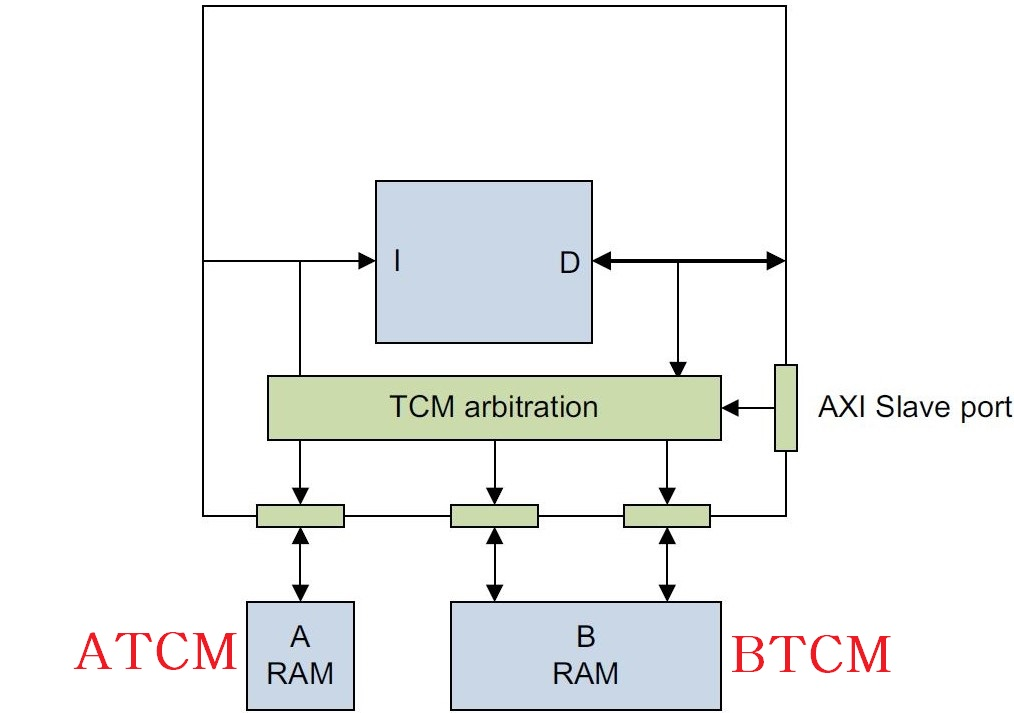
\includegraphics[scale=0.4]{figures/tcm}
%	\caption{}
%	\label{fig:tcm}
%\end{figure}

\begin{wrapfigure}[14]{r}{7cm}
	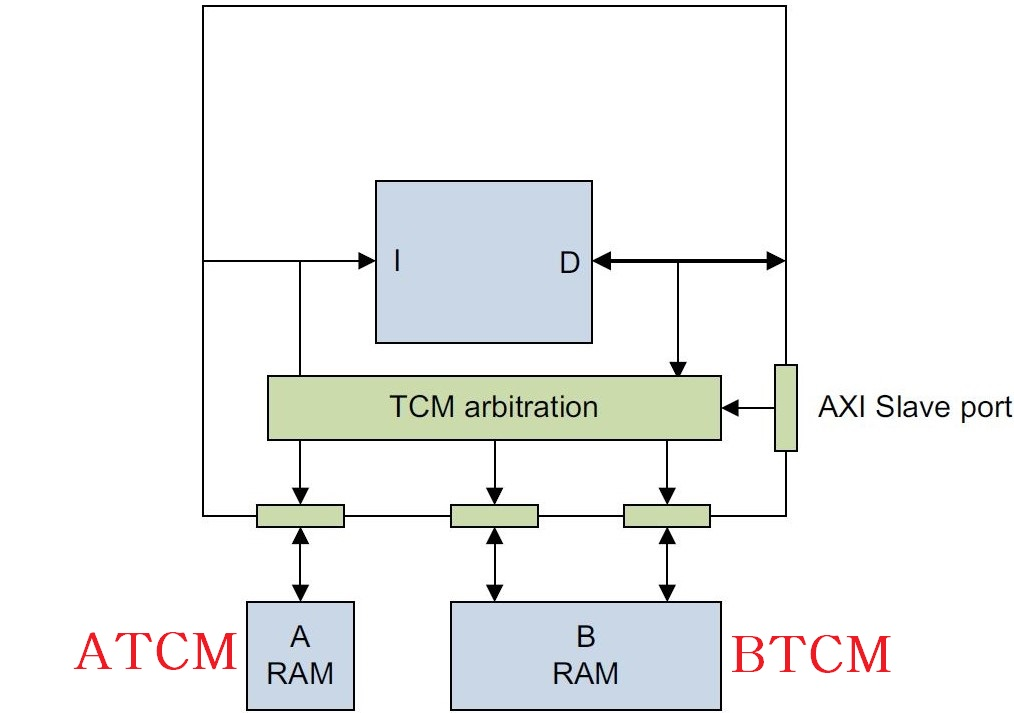
\includegraphics[scale= 0.315]{figures/tcm}
	\caption{TCMs in Cortex-R5} \label{tcm}
\end{wrapfigure}
\paragraph{Tightly-Coupled Memories (TCMs)}  \textit{Unpredictable access time} at a processor request is a common issue related to cache memories because, access times at a \textit{cache hit} and a \textit{cache miss} are different in nature. Tightly-Coupled Memories (TCMs) address this issue and provide \textbf{\textit{low-latency}} memory access and \textbf{\textit{consistent access time}} which is ideal for storing time-critical routines\cite{crspg}. The Cortex-R5 processor can be configured to have one or two TCMs(ATCM \& BTCM) which are located separately from the processor. They may contain any mix of Data and Instructions and can have capacities up to 8MB. These TCMs can be implemented as SRAMs or ROMs and typically fetch data in a single cycle. ATCM has a single port while BTCM has two ports which can be accessed simultaneously as it is implemented as two banks of RAMs. TCMs can be loaded via the \textit{AXI slave port} at Level 2 Interface(shown in figure \ref{r5core}) and processor can fetch instructions from the TCMs directly without going all the way to an external memory. Although the TCM is implemented as a separate RAM it does not have a dedicated \textit{address space}(set of addresses) and it simply \textbf{\textit{uses a portion of the 32-bit address space}} which is used by the processor at normal operation. Therefore when these TCMs are enabled anything at the same address space(as that is allocated for the TCMs) in the external memory is not accessible to the processor\cite{crtrm}.


\subsubsection{Memory Protection Unit(MPU)}

In a multitasking system, the task currently being executed must not affect the system resources(code, data) of the other tasks. This protection mechanism is controlled by the Operating System(OS), typically with the help of both hardware and software. In ARM Cortex-R series processors which implement the ARM \textit{\textbf{Protected Memory System Architecture}}(PMSA) this feature is provided by a dedicated hardware called \textit{Memory Protection Unit}(MPU)\cite{crspg} located inside the \textit{Level 1 Memory System}(shown in figure \ref{r5core}) of the cores. Using the MPU,  memory can be partitioned into \textbf{\textit{zero, 12 or 16 regions}} and protection attributes can be set for each region independently. The size of such a region is specified by a 5-bit value which encodes a range of values from 32-Bytes(cache-line length) to 4GB.\cite{crtrm}
















% arm cr5 2.3.3 Clocking
% Micro Snoop Control Unit (μSCU)
%---------------------------------------------------------
\vspace{1cm}\hrule
\section{Timing related to Memory}

\subsection{Intel Core i3-8300 Processor}
%18.7 COUNTING CLOCKS
In coffee lake $\mu$architecture the processor is divided into several \textbf{\textit{Clock Domains}} where each part maintains a different clock frequency which is applicable only to that part. All of these frequencies are some multiple of what is known as \textit{Base Clock} which acts only as a reference for other clock domains\cite{Skylake} . Cache memories, their related clock domains, latency and bandwidths are as follows. In addition to that system's DRAMs are operated under the \textit{Memory clock} domain and are capable of transferring data at the rate of 8 bytes per cycle per channel\cite{Coffee}(Core i3-8300 Processor is dual channel as mentioned previously).

 \begin{table}[!h]
	\centering
	\begin{tabular}{l| c|c|c|c }
		Cache &Clock Domain&Fastest Latency&Peak Bandwidth&Sustained Bandwidth\\
		&&(cycles)&(bytes/cyc)&(bytes/cyc)\\\hline
		L1 I Cache&Core Clock &N/A&N/A&N/A\\
		L1 D Cache&Core Clock &4&96&81\\
		L2 U cache&Core Clock &12&64&29\\
		L3 U, S Cache/LLC&Ring Clock&44&32&18\\
		\hline\hline
	\end{tabular}
	\caption{Timing Related to Cache Memory in Intel core i3-8300 Processors\cite{iaorm}}
\end{table}

\subsection{Arm Cortex-R5 Processor}
%1.4 Interfaces 9.8 Accelerator Coherency Port interface
In Arm Cortex-R5 Processors there is \textbf{\textit{only one clock}} input(\textbf{\textit{CLKIN}}) for the entire CPU and the \textit{Advanced Microcontroller Bus Architecture}(AMBA) system which consists of AXI master, AXI slave, ACP(Accelerator Coherency Port) and some other ports, is synchronized with this clock. That is even though AMBA system's clock has lower frequency, its rising edge is synchronous to the CLKIN. As mentioned previously, AXI master is used for instruction fetching and data access while AXI slave is used for external access to TCMs. Since ARM Coretx-R5 implements the both \textit{arm} and \textit{thumb-2} ISAs, in ARM state the memory system can supply up to two instructions per cycle while in thumb state the memory system can supply up to four instructions per cycle. In addition to that, access to external memory will take tens or even hundreds of core cycles in a normal ARM processor.

%2.3.3 Clocking



\vspace{1cm}\hrule

\section{Comaprison}

Cortex-R5 is using armv-7r architecture which uses native 32bits data paths, favouring four-byte operations, while intel i3 8300 is using intel’s coffee lake architecture which uses 64bits data paths. Armv-7r is reduced instruction set computing (RISC) based digital logic design and the i3 8300 is complex instruction computing (CISC) based. Simple instructions are operated only on registers and there is a lot of general-purpose registers in cortex-R5. Armv-7r is allowable only read and store with the main memory. The silicon cost is very low, and the power consumption is also very low. The number of general-purpose registers is less in i3 8300 processor and directly operate with main memory as well, while complex instructions are executed in a single clock cycle. There is significant amount of digital logics to manipulate such behaviour. The ALU is directly connected with its 32bits registers and all logical and mathematical operations are manipulated in Cortex-R5. The ALU of i3 8300 is capable of manipulating 64bits numbers and digital logics.  Like other RISC based architectures, this is explicitly fast and widely used in embedded processors. There is a well-known saying that intel architecture is like an American muscle car. It costs more and power-hungry.\\




{\footnotesize \textit{Consider these abbreviations to refer table},
	D-\textit{Data}, I-\textit{Instruction}, WB-\textit{Write-back}, WT-\textit{Write-through} U-\textit{Unified}, S-\textit{Shared}, SA-\textit{Set Associative}}

\begin{table}[!h]
	\centering
	\begin{tabular}{l ||c| c }
		\textbf{Feature} &\textbf{ARM cortex-R5}&\textbf{Intel Core-i3-8300}\\\hline
		ISA &RISC&CISC\\
		Micro Architecture &ARMv7r&Coffee Lake($8^{th}$ Gen: Intel)\\
		Digital logic design&	Comparably simple	&Complex\\
		Silicon cost&	Low	&High\\
		Operation	&Only on registers&	On registers \& directly on memory as well\\
		Data paths&	32 bits	&64 bits\\

		Number of Cores& Single/Dual(Configurable)&4\\
		Memory Sys: Archi:&Protected Mem: Sys: Archi:(PMSA)&Virtual Mem: Sys: Archi:(VMSA)\\
		TLBs&N/A&I-TLB, D-TLB, STLB-U\\
		%Typical clock speed&600 MHz on 40 nm&\\
		Cache  Levels& L1-I, L1-D, Optional L2  & L0-$\mu$OP, L1-I,   L1-D, L2-U, L3-U-S\\
		Cache Mapping Technology&Set Associative&Set Associative\\
		Cache writing Policy&WB or WT (Configurable through MPU)& WB\\
		Cache Line Size&32 Bytes&64 Bytes\\
		TCMs&Single Port ATCM, Dual Port BTCM&N/A\\
		Primary(physical) DRAM& 4GB&Upto 64GB of DDR4-2400\\
		ECC on Memories& Available& Available\\
		Clock Domains& Single Clock Input(CLKIN)&Multiple Clock Domains\\


		\hline\hline
	\end{tabular}
	\caption{Key differences in two processors}
\end{table}





%Arm Cortex-R5 Processor Intel Core i3-8300 Processor

%\paragraph{Instruction Set Architecture of the Processor}
%\paragraph{Micro-Architecture (Data Path and the Controller)}
%\paragraph{ALU functions}
%
%\paragraph{Cache Memory and Memory Interfacing} In the given two processors there are strong differences in cache memory organization. In Intel Core i3-8300 Processor there are 4 levels of cache while there is only L1 cache  in the Arm Cortex-R5 Processor since L2 cache is optional.
%
%\paragraph{Timing related to Memory}


\vspace{1cm}\hrule
\bibliographystyle{plain}
\scriptsize
\bibliography{reference}
%
\end{document}
